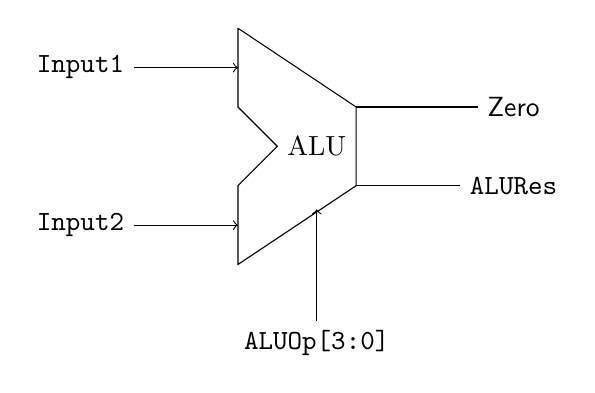
\begin{tikzpicture}

\draw (-1,1.5) -- (-1,0.5) -- (-0.5,0) -- (-1,-0.5) -- (-1,-1.5) -- (0.5,-0.5) node (v5) {} -- (0.5,0.5) node (v3) {} -- (-1,1.5);
\node at (0,0) {ALU};
\node[font=\ttfamily] (v1) at (-3,1) {Input1};
\node[font=\ttfamily] (v2) at (-3,-1) {Input2};
\draw (v1) edge[->] (-1,1);
\draw (v2) edge[->] (-1,-1);
\node[font=\sffamily] (v4) at (2.5,0.5) {Zero};
\draw  (0.5,0.5) edge (v4);
\node[font=\ttfamily] (v6) at (2.5,-0.5) {ALURes};
\draw  (0.5,-0.5) edge (v6);
\node[font=\ttfamily] (v7) at (0,-2.5) {ALUOp[3:0]};
\draw (v7) edge[->] (0,-0.8);
\end{tikzpicture}